\chapter{Обзор литературы} \label{chapt1}

\section{Современное состояние исследований оптических частотных гребенок в микрорезонаторах} \label{sect1_1}

Открытие и развитие оптических частотных гребенок на основе фемтосекундных лазеров с синхронизацией мод оказало огромное влияние на науку и технологии с момента их первоначальной демонстрации в 2000 году \cite{Jones635,PhysRevLett.84.5102}. Это открытие было отмечено Нобелевской премией по физике в 2005 г \cite{Hall2006}. Помимо приложений в прецизионной частотной метрологии и для создания атомных часов \cite{Diddams2001,Udem2002,Ye2005,Diddams2004}, возможность эффективного контроля амплитуды и фазы точно определенных спектральных линий открыла новые подходы для генерации аттосекундных импульсов, спектроскопии веществ \cite{Stowe2008,Diddams2007,Ideguchi2013,Holzwarth2000}, обработки оптических сигналов и радиофотоники \cite{Gao2006,Torres2014}, калибровки астрономических эшелле-спектрографов \cite{Steinmetz2008} и синтеза спектрально чистых СВЧ сигналов \cite{Fortier2011}.

Открытые в лаборатории профессора Т. Киппенберга в 2007 году оптические частотные гребенки в микротороидах из плавленого кварца \cite{DelHaye2007} вызвали новую волну интереса и исследований в области микрорезонаторов и частотной метрологии \cite{Kippenberg2011}. Оптическая частотная гребенка в микрорезонаторе представляет собой набор эквидистантных спектральных линий, получающихся каскадно при накачке высокодобротной моды пассивного микрорезонатора из материала с кубичной нелинейностью с помощью мощного, узкополосного и перестраиваемого лазера непрерывной мощности. Керровские частотные гребенки имеют расстояния между линиями 5-1000 ГГц и позволяют достичь уровня миниатюризации и энергоэффективности устройств, труднодостижимого для гребенок, полученных с помощью фемтосекундных лазеров с синхронизации мод. Над развитием этой новой области работают около 10 экспериментальных групп и еще несколько теоретических групп. За 11 прошедших с открытия лет был проведен обширный теоретический анализ и численное моделирование богатой нелинейной динамики процесса формирования оптических гребенок. В отличие от частотных гребенок, получаемых при синхронизации мод фемтосекундного лазера, произвольные оптические частотные гребенки из микрорезонатора не представляют собой короткие импульсы во временном представлении из-за произвольных фазовых соотношений между отдельными спектральными линиями, появляющимися в процессе каскадного формирования гребенки \cite{Herr2012}.

Некогерентные шумные оптические гребенки были продемонстрированы в различных структурах, в том числе в кристаллических резонаторах из различных фторидов при накачке в ближнем ИК \cite{Savchenkov2008,Grudinin2012,Liang2011,Grudinin2009,Henriet:15}, в том числе шириной в октаву \cite{DelHaye2011}, в интегральных микрорезонаторах из нитрида кремния ($Si_3N_4$) \cite{Levy2010,Okawachi2011,Johnson2012,Huang2015}, в планарных системах, изготовленных из стекла Hydex \cite{Moss2013,Razzari2010}, а также в других диэлектрических материалах: нитриде алюминия $AlN$ \cite{Jung2013}, фосфиде галлия $GaP$ \cite{2018arXiv180803554W} и алмазе \cite{Hausmann2014}. Важным типом резонаторов являются кольцевые волоконные резонаторы ($SiO_2$), в которых динамика гребенок описывается теми же уравнениями, и возможно прямое измерение профиля поля внутри резонатора благодаря длительности импульса $5-10$ пс. Именно в волоконных кольцевых резонаторах было впервые продемонстрировано формирование и распространение солитонов, но при накачке затравочным импульсом \cite{Leo2010}.

Большим прорывом стало теоретическое предсказание и экспериментальная демонстрация высококогерентных частотных гребенок, линии которых синхронизированы по фазе \cite{Herr2014}. Такая малошумная оптическая гребенка соответствует оптическому временному солитону, распространяющемся внутри микрорезонатора. Для стационарного режима распространения солитонов необходим баланс между дисперсией групповой скорости и нелинейностью в микрорезонаторе, а также между потерями и накачкой через параметрическое преобразование частоты. Предложенный метод основан на перестройке частоты лазера накачки из области синей отстройки от моды микрорезонатора в красную сторону, в область существования солитона. Этот метод позволил генерировать когерентные и широкополосные оптические гребенки, которые могут быть достигнуты повторяемо. Эта работа показала возможность генерации фемтосекундных оптических импульсов с малым джиттером из вакуумных флуктуаций мод микрорезонатора. C помощью этого метода оптические солитоны были получены в кристаллических цилиндрических \cite{Herr2014} и кварцевых микротороидах \cite{Yi2015} при накачке на длине волны около $1550$ нм. В этих же двух работах было произведено частотно-разрешенное оптическое стробирование (FROG) для экспериментального подтверждения импульсного временного профиля электрического поля в микрорезонаторе. В работе \cite{Brasch2016} впервые показали формирование оптического солитона и генерацию высоко когерентной гребенки спектральной шириной в $2/3$ октавы в $Si_3N_4$ кольцевом микрорезонаторе, интегрированном на чип. Также солитонная гребенка была продемонстрирована в интегральном кольцевом резонаторе из кремния $Si$ при накачке в среднем ИК диапазоне, где двухфотонное поглощение в материале мало \cite{Yu2016}, настройка на солитонный режим достигался путем инжекции свободных носителей в PIN структуру и мониторинга тока на ней. Недавняя работа показала возможность генерации оптических солитонов в интегральном резонаторе из ниобата лития $LiNbO_3$, где квадратичная нелинейность не равна нулю, так что одновременно с солитонной гребенкой с центром на 1550 нм образовывалась гребенка на удвоенной частоте 775 нм. Таким образом по состоянию на конец 2018 г. солитонный режим оптических гребенок был продемонстрирован в меньшем количестве материалов ($MgF_2, Si_3N_4, Si, SiO_2, LiNbO_3$), чем шумная оптическая гребенка.
 
Обширное описание работ, посвященных оптическим гребенкам и солитонам в микрорезонаторах даны в обзорах \cite{Kippenberg2011,ASavchenkov2016,ChemboY2016,PASQUAZI20181,Kippenbergeaan8083}

В последнее время появилось множество работ, посвященных генерации и свойствам солитонов в микрорезонаторах  \cite{Godey2014,Jaramillo2015,Jang2015,Hansson2016,Lamont2013,Saha2013,Matsko2012,DelHaye2014,Wang2014,Bao2014,Chembo2010}.


В работе \cite{Jost2015} продемонстрирована солитонная гребенка из микрорезонатора и привязка лазера накачки к стабилизированной гребенке из фемтосекундного лазера, тем самым достигается полностью стабилизированная оптическая гребенка из кристаллического микрорезонатора.


В работе \cite{HerrPRL2014} описаны механизмы, препятствующие образованию солитонов в микрорезонаторах: большая по модулю дисперсия групповой скорости и эффекты нормального расщепления мод вблизи моды накачки.


Возможность синтезировать частотные гребенки непосредственно на чипе открывает путь к полностью интегрированным генераторам оптических гребенок, которые могут существенно упростить процессы измерения и синтеза частоты, и, тем самым, выйти на коммерческий рынок. Основными преимуществами частотных гребенок из микрорезонаторов являются их компактность, высокая мощность, приходящаяся на каждую компоненту гребенки, и возможность получения частот повторения в диапазоне 10-1000 ГГц, важном для многих приложений, включая телекоммуникации высокой пропускной способности \cite{Pfeifle2014}, астрофизику \cite{Glenday2015}, синтез частот \cite{Ferdous2011}, радиофотонику и генерацию микроволн \cite{Xue2016,Savchenkov2008}. Оптическая частотная гребёнка может быть использована как высокостабильный калибровочный репер для прецизионной спектроскопии, как источник спектрально чистого СВЧ сигнала, а также для генерации фемтосекундных оптических импульсов – генераторы гребенки могут обеспечивать короткие периодические оптические импульсы (солитоны длительностью ~300 фс в кристаллических и 20 фс в интегральных) с очень малым временным джиттером. Параметрический характер усиления обеспечивает широкополосность процесса в полосе, достигающей октавы. Подобный спектр гребенки может связывать оптический диапазон с микроволновым и наоборот. Кроме того, ширина полосы усиления ограничена только окном прозрачности материала микрорезонатора, что позволяет генерировать гребенки как в УФ, так и среднем ИК диапазонах.

В то же время в последние несколько лет было предложено несколько перспективных методов, позволяющих обойтись без быстрой перестройки частоты лазера накачки для генерации солитонного режима: один из них базируется на использовании фазомодулированной накачки \cite{Taheri2015,Jang2015ol}, а второй – на тепловых эффектах \cite{Kobatake2016}, в том числе и с использованием дополнительного нагревательного элемента \cite{Joshi2016}. При нагреве микрорезонатора происходит сдвиг резонансных частот микрорезонатора относительно частоты накачки, что в какой-то мере эквивалентно ранее описанному процессу перестройки частоты лазера накачки. Также было показана возможность получения односолитонного режима, важного для практических применений. Это осуществлялось либо контролируемым нагревом и охлаждением нагревательного элемента, либо обратной медленной перестройкой частоты лазера накачки \cite{Karpov2017}. Также недавно был продемонстрирован метод генерации солитонов с помощью интегрированных PIN-структур, позволяющих контролировать время жизни свободных носителей заряда \cite{Yu2016}.

Одной из приоритетных задач в области микрорезонаторных частотных гребенок является расширение спектрального покрытия существующих керровских гребенок. Перспективным направлением исследований является генерация керровских частотных в среднем ИК диапазоне. Этот диапазон интересен тем, что в нем находятся колебательные уровни многих молекул, из-за чего его называют диапазоном “молекулярной дактилоскопии” \cite{Diddams2007}. К таким молекулам относятся углеводороды, вещества, важные для экологии, токсичные химикаты. В настоящее время средний ИК изучается в основном с помощью инфракрасных-Фурье спектрометров (ИКФС) \cite{Griffiths2006}. Оптические гребенки в среднем ИК могут представлять собой очень интересное технологическое решение для молекулярной дактилоскопии, а компактный источник частотной гребенки в среднем ИК может обеспечить значительный потенциал для расширения возможностей и областей применения среднего ИК диапазона. С одной стороны, он может быть использован в качестве яркого источника для Фурье-спектрометра. 

Тем не менее, технология генерации керровских гребенок в среднем ИК остается сравнительно слаборазвитой и количество публикаций, посвященных этой проблеме, сравнительно мало \cite{Schliesser2012,Wang2013,Griffith2015,Griffith2016,Savchenkov2015}. В частности, в экспериментах, проведенных в EPFL при использовании параметрического лазера непрерывного излучения в качестве накачки, была показана возможность генерации оптических гребенок в среднем ИК на длине волны 2.5 мкм \cite{Wang2013}. Генерация в среднем ИК также была продемонстрирована в структурах из нитрида кремния \cite{Griffith2015,Griffith2016}. Также генерация гребенки со спектральной шириной, превышающей половину октавы, была продемонстрирована в микрорезонаторах из $CaF_2$ и $MgF_2$ при накачке квантово-каскадным лазером \cite{Savchenkov2015}. В основном же для генерации гребенок в среднем ИК успешно применялись такие подходы, как параметрическая генерация или генерация разностной частоты \cite{Adler2009,Leindecker2011,Maddaloni2006,Cruz2015}, однако ширина полосы и величина мощности, приходящейся на каждую компоненту гребенки, а также степень когерентности остаются ограниченными так же, как и габариты экспериментальной установки. В качестве материала, пригодного для генерации частотных гребенок в среднем ИК, в последнее время изучались фториды бария, стронция и кальция \cite{Grudinin2016,Lin2015,Way2012,Lecaplain2016}.


Более интересной является перспектива использования таких компактных устройств для спектроскопии с использованием двух оптических гребенок (будем далее для краткости называть двухгребеночная спектроскопия) \cite{Ideguchi2014,Coddington2016,Suh2016}, когда сбиваются два источника гребенок в среднем ИК с различными частотами повторения, и генерируется сигнал биений на фотодетекторе в форме гребенки, но уже в радио диапазоне частот, что может быть использовано для восстановления профилей поглощения веществ в быстром, компактном устройстве без подвижных механических частей.


Еще одним чрезвычайно важным направлением исследований является возможность генерации когерентных гребенок в режиме нормальной дисперсии \cite{Xue2016nano}, т.е. в видимом и ближнем ИК диапазоне длин волн, т.к. материальная дисперсия большинства исследуемых материалов в этих диапазонах является нормальной. Что касается видимого диапазона \cite{Miller2014,Jung2014}, следует отметить, что керровские частотные гребенки с большим межмодовым расстоянием могут, в частности, использоваться для астрофизических измерений \cite{Benedick2010,Glenday2015} и приложений рамановской спектральной визуализации. Также возможно применение керровских гребенок в видимом диапазоне и ближнем ИК для двухгребеночной спектроскопии \cite{Zhu2013}. Видимый диапазон привлекателен еще и тем, что в нем возможна визуализация биологических веществ из-за наличия в нем окна спектра пропускания воды, и он также характеризуется большими сечениями комбинационного рассеяния. Отметим, что в основном до настоящего времени для генерации частотных гребенок в видимом диапазоне использовалось совместное действие квадратичной и кубичной нелинейностей \cite{Miller2014,Jung2014}.


Из-за наличия пиков поглощения в УФ многие диэлектрические материалы имеют нормальную дисперсию групповых скоростей (ДГС) в видимом диапазоне и ближнем ИК, что препятствует генерации светлых солитонов. Теоретически и экспериментально узкие керровские частотные гребенки при нормальной ДГС изучались в кристаллических микрорезонаторах \cite{Coillet2013,Liang2014,Henriet2015} и микрокольцах на чипе \cite{Huang2015prl}. Также было теоретически и экспериментально продемонстрировано существование темных временных импульсов \cite{Godey2014,Xue2015,Lobanov2015,ParraRivas2016}. В частности, в ряде работ существование темных солитонов было связано с наличием волн переключения между двумя плосковолновыми состояниями \cite{ParraRivas2016}. Однако на сегодняшний день полное понимание динамики этого процесса, в том числе механизмов, обеспечивающих генерацию керровских частотных гребенок с малым шумом в режиме нормальной дисперсии, отсутствует. %  TODO: add dark breathers 
Было показано, что в системе с двумя связанными микрорезонаторами этим взаимодействием можно управлять \cite{Liu2015}. 

% TODO: Перенести в главу
Также, недавно было численно показано, что мягкое возбуждение платиконов возможно и без модификации закона дисперсии при двухчастотной накачке или при достаточно сильной амплитудной модуляции накачки с разницей частот кратной области свободной дисперсии резонатора (ОСД) \cite{Lobanov2015epl}. Применимость этой методики подтверждается тем, что ранее при ее помощи теоретически \cite{Hansson2014} и экспериментально \cite{Strekalov2009} была продемонстрирована генерация керровских частотных гребенок в режиме аномальной дисперсии. Также недавно была продемонстрирована генерация частотной гребенки в оптоволокне с нормальной дисперсией при двухчастотной накачке \cite{Antikainen2015}.
%

Еще одним актуальным направлением исследований в области микрорезонаторных частотных гребенок является разработка методов увеличения их ширины и когерентности. Одним из исследуемых в последнее время способов является взаимодействие временных солитонов и дисперсионных волн (иногда по аналогии с классическим эффектом Черенкова называемых, индуцированным  солитонами черенковским излучением) \cite{Brasch2016,Akhmediev1995,Barashenkov2011,Jang2014,Milian2014,Yang2016}. При накачке микрорезонатора в области аномальной дисперсии возможна генерация светлого солитона. Если его длительность достаточно мала, то его спектр распространяется в область нормальной дисперсии и солитон может генерировать дисперсионную волну – пик излучения вблизи точки нулевой дисперсии. Формирование дисперсионной волны в присутствии солитона может способствовать уширению полосы генерации гребенки в область нормальной дисперсии без потери когерентности. Таким способом была экспериментально продемонстрирована генерация гребенки шириной в 2/3 октавы в микрорезонаторе, интегрированном на чип при накачке на длине волны 1.55 мкм \cite{Brasch2016}.


Для генерации и реализации эффективного взаимодействия солитонов и дисперсионных волн должны выполняться определенные дисперсионные соотношения, поэтому разрабатывается множество методов получения оптимальной дисперсии (dispersion engineering). Дисперсия кристаллического резонатора может быть специально задана \cite{Grudinin2012,Jiang2014,Okawachi2014,Zhang2014,Zhang2013,Grudinin2015,Nakagawa2016}, например, с помощью микроструктурирования его формы \cite{Grudinin2015,Nakagawa2016}. В частности, было продемонстрировано, что эффективно изменять дисперсию можно путем прецизионного формирования микрометрических выступов \cite{Grudinin2015}. Также специально рассчитанная форма поперечного сечения микрорезонатора может обеспечить аномальную дисперсию в диапазоне, превышающем октаву \cite{Nakagawa2016}.

%TODO: обзор ТГц гребенок, октавная с 2мя дисперсионными волнами + оптический синтезатор частот

Большой интерес привлекает возможность использования эффектов рамановского и бриллюэновского рассеяния для генерации частотных гребенок и контроля их свойств. Например, активно исследуется влияние рамановского рассеяния на генерацию и свойства диссипативных солитонов в оптических микрорезонаторах (например, эффект сдвига спектрально максимума солитона, Raman induced soliton self-frequency shift) \cite{Hansson2014ol,Milian2015,Yi2016,Karpov2016,Bao2017}. Также в нескольких недавних работах \cite{Chembo2015,Chembo2016} исследовалась возможность генерации оптической частотной гребенки в полосе рамановского рассеяния в области нормальной дисперсии групповой скорости, где обычные методы работают плохо. В работе \cite{Chembo2015} экспериментально была продемонстрирована генерация оптической частотной гребенки в кристаллическом резонаторе из MgF2 при накачке 1064 нм в присутствии интенсивного спектрального максимума, вызванного вынужденным комбинационным рассеянием. Это было интерпретировано авторами как совместное воздействие эффектов Рамана и Керра (Kerr-Raman interaction). Этот результат открывает новый путь к генерации оптических частотных гребенок в области нормальной дисперсии групповой скорости. Однако теоретические выводы авторов основанные на численном решении уравнения Луджиато-Лефевра значительно расходятся с экспериментальными результатами и не позволяют в полной мере проанализировать процесс генерации гребенки и ее когерентные свойства.



Важной задачей является разработка новых устройств для генерации микрорезонаторных гребенок на едином чипе. Одной из конструкций может быть микрорезонатор, связанный через затухающее поле, например, с экситонами в квантовых ямах с электрической или оптической накачкой. Эта система может работать в режимах сильной связи, когда образуются поляритоны \cite{Schneider2013}. Поляритоны существуют в относительно узком спектральном диапазоне вблизи экситонного резонанса, где накачка и сильная поляритонная нелинейность включают процесс параметрического преобразования, который запускает генерацию широкой гребенки уже в фотонном (неполяритонном) режиме. Идея связи микрорезонатора с усилителем недавно была проверена в эксперименте, в котором микрорезонатор был помещен в виток волоконного усилителя (EDFA) и была получена гребенка \cite{Johnson2014}. Недавняя теоретическая работа по поляритонным гребенкам рассматривала модель узкой резонансной полосы частот, где могут существовать лишь несколько спектральных линий \cite{Rayanov2015}.


Рассмотрим более подробно основные достигнутые результаты по генерации оптических частотных гребенок и солитонов, их количественные характеристики и основные продемонстрированные применения.

Первое экспериментальное наблюдение оптического гребенок в микрорезонаторах было продемонстрировано в 2007 году в работе \cite{DelHaye2007}. Использовался резонатор в форме тороида из плавленого кварца, размещенный на кремниевой подножке. Добротность резонатора составила $Q=10^8$. Связь с резонатором осуществлялась с помощью растянутого оптоволокна. Накачка проводилась непрерывным лазером на длине волны $1550$ нм и мощностью $50$ мВт. Наблюдалась генерация боковых мод в сторону больших и меньших частот от накачки. За счет процессов четырехволнового взаимодействия гребенка расширялась. Для тороида диаметром $75$ мкм возбуждалось более 70 мод, почти равномерно покрывающих диапазон в $500$ нм. Для резонатора большего диаметра ($190$ мкм) наблюдалась гребенка шириной $380$ нм, содержащая 134 моды, с межмодовым интервалом $375$ ГГц. Был проведен эксперимент по проверке эквидистантности мод полученной гребенки путем сравнения ее с эталонной гребенкой, генерируемой импульсным лазером в нелинейном волокне (по методу Т. Хэнша). Равномерное распределение мод (эквидистантность) была подтверждена с высокой точностью. В работе проведено измерение дисперсии, она положительна, т.к. материальная дисперсия $\Delta\nu_{FSRmat}$ в плавленом кварце компенсирует отрицательную геометрическую дисперсию $\Delta\nu_{FSRgeom}$. Дисперсия групповой скорости $GVD$ в плавленом кварце положительная для длин волн больших $1.3$ мкм.

\begin{equation}
\Delta\nu_{FSR}=(\nu_{m+1}-\nu_m)-(\nu_m-\nu_{m-1}),
\end{equation}
\begin{equation}
\Delta\nu_{FSRgeom}\approx-0.41\frac{c}{2\pi nR}m^{-\frac{5}{3}},
\end{equation}
\begin{equation}
\Delta\nu_{FSRmat}\approx\frac{c^2\lambda^2}{4\pi^2n^3R^2}GVD,
\end{equation}
\begin{equation}
GVD=-\frac{\lambda}{c}\frac{\partial^2 n}{\partial \lambda^2},
\end{equation}
где $\nu_m$ - частота моды с номером $m$, $c$ - скорость света, $n$ - показатель преломления среды, $R$ - радиус резонатора, $\lambda$ - длина волны.

В работе \cite{DelHaye2011} продемонстрирована генерация октавной гребенки. Этого удалось добиться за счет оптимизации дисперсии резонатора (путем численного моделирования его геометрии), увеличения его добротности и мощности лазера накачки. Экспериментальная установка состоит из диодного лазера, сигнал которого усиливается эрбиевым волоконным усилителем (EDFA) до выходный мощности $2.5$ Вт. Связь с резонатором осуществляется через растянутое волокно. Из-за большой мощности накачки моды резонатора испытывают термический сдвиг, требуя большой перестройки лазера накачки (до $1$ ТГц), чтобы оставаться в резонансе с модами микрорезонатора. Гребенка наблюдается с помощью двух оптических спектроанализаторов. При накачке на частоте $1560$ нм в резонаторе наблюдается спектр гребенки, покрывающий одну октаву (рис. \ref{octave_comb_mlg}). Для резонатора диаметром $80$ мкм и добротностью $Q\approx2.7\times10^8$ межмодовое расстояние гребенки составляет $850$ ГГц. Измеренное значение ширины линии гребенки $\approx 70$ МГц. В работе продемонстрирована возможность перестройки лазера накачки более, чем на одну область свободной дисперсии (до $500$ ГГц) с сохранением генерации октавной гребенки, покрывающей диапазон $140-280$ ТГц.
\begin{figure}
  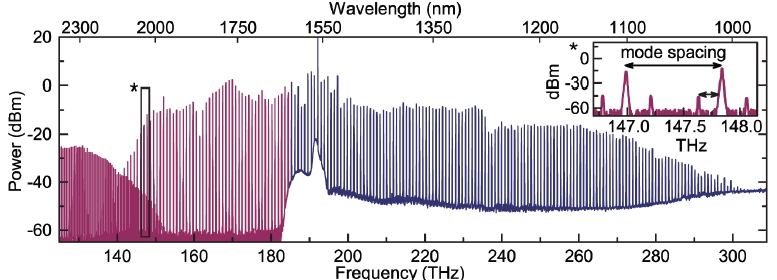
\includegraphics[]{octave_comb_mlg}
  \caption{Спектр октавной гребенки, полученной из тороидального резонатора из плавленого кварца диаметром $40$ мкм. Расстояние между линиями гребенки $850$ ГГц. Взято из \cite{DelHaye2011}}
  \label{octave_comb_mlg}
\end{figure}


В работе \cite{Herr2012} экспериментально изучалась динамика генерации гребенок в двух различных резонаторах: $MgF_2$ (ширина резонанса $1$ МГц), и $Si_3N_4$ (200 МГц). Геометрии резонаторов изображены на рис. \ref{mgf2_si3N4_resonators}.

\begin{figure}
  \centering
  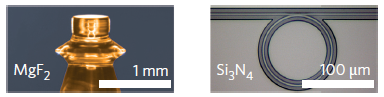
\includegraphics[]{mgf2_si3N4_resonators}
  \caption{Форма резонаторов, в которых наблюдались оптические гребенки. Взято из \cite{Herr2012}}
  \label{mgf2_si3N4_resonators}
\end{figure}
Для генерации первых боковых мод и далее всей гребенки лазер накачки постоянной мощности изначально сильно отстроен в синюю область от резонансной моды. Далее отстройка накачки медленно уменьшается, так что все больше и больше света связывается с резонансом. В некоторой точке достигается параметрический порог и возникает первая пара боковых мод. Экспериментальный вид спектра гребенок для обоих резонаторов представлен на рис. \ref{universal_formation_mlg}. Рассматриваются 2 сценария развития гребенки: а) первые образовавшиеся боковые моды являются соседними к моде накачки резонатора; б) первые боковые моды образуются вдалеке (по номеру моды) от накачки. Используется разложение собственных мод невозбужденного резонатора $\omega_\mu=\omega_0+D_1\mu+\frac{1}{2}D_2\mu^2$, где $D_1$ соответствует ОСД резонатора, $D_2$ - разность двух соседних ОСД около центральной частоты $\omega_0$. Далее аналитически решается система связанных уравнений для двух боковых мод и моды накачки. Собственные значения этой системы дают условие на порог генерации боковых мод. Откуда можно получить выражение для минимального номера первично возбуждаемых мод $\mu_{th,min}=\sqrt{\frac{\kappa}{D_2}}$, где $\kappa$ обозначает суммарные потери в резонаторе и элементе связи.
\begin{figure}
  \centering
  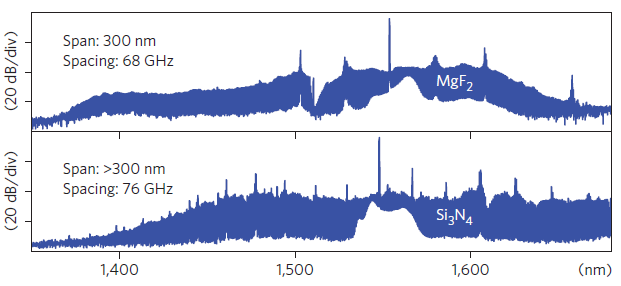
\includegraphics[]{universal_formation_mlg}
  \caption{Спектр наблюдаемых гребенок. Мощность накачки для $MgF_2$ - $500$ мВт; для $Si_3N_4$ - $3$ Вт. Взято из \cite{Herr2012}}
  \label{universal_formation_mlg}
\end{figure}

В работе \cite{Chembo2010pra} приводится общее описание сферических микрорезонаторов с модами типа шепчущей галереи (МШГ), дается вывод системы связанных уравнений (спектральное представление), описывающих динамику каждой моды. Аналитически выводится значение пороговой мощности, необходимой для начала генерации гребенки $P_{th}=\frac{n_0^2 V_0}{2\hbar\omega_0 n_2 c Q_0}$, где $n_0$ - показатель преломления, $V_0$ - эффективный объем моды, $\omega_0$ - частота накачки, $Q_0$ - собственная добротность резонатора, $n_2$ - нелинейная часть показателя преломления. В статье проведено численное моделирование этой системы для $200$ мод.

Оптические гребенки наблюдались при разных геометриях резонаторов и разных типах связи с ними. В работе \cite{DelHaye2013} из цилиндрической заготовки из кварца при ее вращении выжигались $CO_2$ лазером резонаторы в форме микрокольца вокруг цилиндра диаметром от $170$ мкм до $8$ мм. В этих резонаторах удалось генерировать гребенку с расстоянием между модами от $300$ ГГц до $8.4$ ГГц соответственно. В работе \cite{Wang2013oe} использовался планарный кольцевой резонатор из нитрида кремния с использованием второго волновода для выходящего сигнала, при этом спектр на выходе был более гладким, т.к. спектральная линия большой мощности накачки не попадала в дроп-порт.

Другой подход к моделированию оптических частотных гребенок основан не на системе связанных уравнений в спектральном представлении, а на решении уравнения Луджиато-Лефевера в пространственно-временном представлении.

В работах \cite{Matsko2011} и \cite{Chembo2013} дан вывод этого уравнения из уравнений связанных мод. Решение уравнения Луджиато-Лефевера описывает в данном случае диссипативный временной солитон, распространяющийся в резонаторе. Экспериментальное наблюдение солитонов впервые было продемонстрировано в статье \cite{Herr2014}. Длительность солитона (полная ширина на половине высоты) составила около $200$ фс, период их следования около $28$ пс (для односолитонного режима). Экспериментальные данные первой демонстрации солитонов представлены на рис. \ref{experiment}

\begin{figure}
  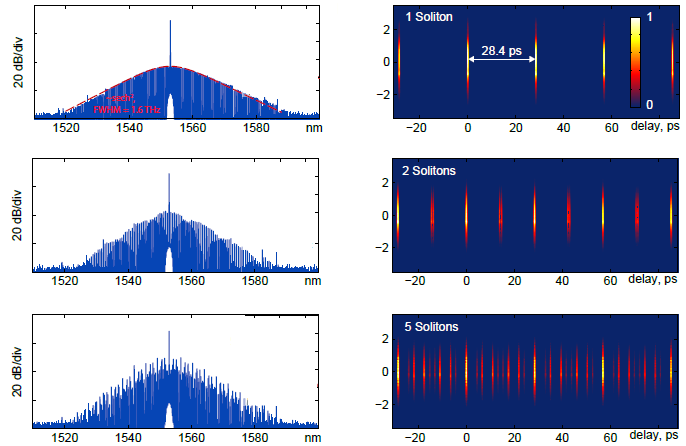
\includegraphics[]{experiment}
  \caption{Экспериментально полученный спектр гребенки для одно-, двух и пяти солитонного режимов. Справа картина соответствующих импульсов во временном представлении. Взято из \cite{Herr2014}} \label{experiment}
\end{figure}

Обзор потенциальных применений оптических гребенок в микрорезонаторах дан в \cite{Kippenberg2011}. Используя компактные микрорезонаторы и один лазер накачки, можно сделать калибровку для астрономического спектрографа для видимого и ближнего ИК диапазонов, с межмодовым расстоянием $10-30$ ГГц. Такие устройства могут позволить измерить доплеровский сдвиг в спектре звезды с точностью, требуемой для обнаружения планет вне Солнечной системы. Ключевым преимуществом в этом случае является малый размер и масса системы.

Гребенки в микрорезонаторах могут использоваться в прямой спектроскопии атомов и молекул по тем же методам, что были разработаны для оптических гребенок с использованием фемтосекундного лазера (по Т. Хэншу). В установке используются две гребенки (которые могут располагаться на одном чипе), имеющие немного различные межмодовые интервалы. Одна гребенка используется как локальный осциллятор, другая используются для получения оптической спектральной картины исследуемого образца. Результирующие биения двух гребенок дают радиочастотный сигнал, содержащий информацию о линиях поглощения. Первая демонстрация спектроскопии с использованием двух солитонных гребенок из двух отдельных микрорезонаторов из плавленного кварца была дана в \cite{Suh2016}, оптические гребенки шириной 4 ТГц с центром на 1.5 мкм были перенесены в радиодиапазон, проведена спектроскопия произвольного сигнала вейвшейпера (оптического генератора сигнала произвольной формы) и линий поглощения ячейки с $HCN$. Оптическое разрешение составило 22 ГГц, равное межмодовому расстоянию солитонной гребенки.

Генерация оптических гребенок с высокой мощностью на каждую линию ($>1$ мВт) и межмодовым интервалом в $10,25,50,100$ ГГц может использоваться в многоканальной оптической телекоммуникации на частотах $1450-1750$ нм. Микрорезонатор и один мощный лазер может заменить индивидуальные лазеры для каждого телекоммуникационного канала. В работе \cite{Pfeifle2014} экспериментально продемонстрировано использование оптических гребенок в микрорезонаторе в роли оптического источника в установке для спектрального уплотнения телекоммуникационных каналов и когерентной передачи данных с использованием амплитудно- и фазово0 модулированных несущих. Достигнута пропускная способность $392$ Гбит/с.

Другим применением могут быть оптические часы. Экспериментальная демонстрация таких часов дана в \cite{Papp2014}. Модулированный по амплитуде лазер с максимальной мощностью $140$ мВт возбуждает кольцевой резонатор из плавленного кварца (расположен на чипе, добротность $Q=6\times10^7$). Генерируется гребенка, покрывающая $20$ нм интервал около накачки $1560$ нм. Межмодовое расстояние составило $33$ ГГц. Далее гребенка расширяется до $200$ нм при ее пропускании через сильно нелинейное волокно. Новый спектр покрывает частоту рубидиевого стандарта (после удвоения частоты). Выбираются две линии гребенки на расстояний 108 мод друг от друга ($1560$ и $1590$ нм соответственно), которые привязываются через дополнительные лазеры к рубидиевым переходам. Выходным сигналом часов является разность частот этих двух стабилизированных лазеров. Она составила $32.9819213$ ГГц. Девиация Аллана достигала $5\times10^{-11}$ при измерении за $10^4$ сек.

В работах \cite{Herr2012}, \cite{Savchenkov2008} продемонстрирована возможность генерации СВЧ сигналов с малым шумом, используя оптические частотные гребенки. Частота СВЧ сигнала определяется межмодовым интервалом гребенки.
%Установка \cite{Herr2014} для наблюдения оптических гребенок (рис. \ref{scheme}) состоит из лазера с узкой линией, работающего в непрерывном режиме генерации, используемого для накачки микрорезонатора из нелинейного материала. Связь с резонатором происходит через срезанное под острым углом или растянутое волокно, призму. Гребенки наблюдаются с помощью анализатора спектра. Используется резонаторы в форме тороида, сферы или диска \cite{Kippenberg2011}. Гребенки наблюдались для резонаторов с добротностью $10^7-10^9$ \cite{Herr2012} и для резонаторов в интегральном исполнении с добротностью $10^6$.



